\section{Resultados}

En la tabla \ref{table:parameters} se encuentran los parámetros ingresados para el algoritmo de descenso del gradiente para la función log-likelihood.

\begin{table}[H]
    \centering
    \begin{tabular}{ccc} \hline
        $c_1$       & $c_2$ & Tolerancia  \\   \hline
        $1x10^{-4}$ & 0.9   & $1x10^{-6}$ \\ \hline
    \end{tabular}
    \caption{Parámetros usados para el algoritmo \ref{alg:alpha_algorithm} con la función log-likelihood.}
    \label{table:parameters}
\end{table}

En la figura \ref{fig:log_likelihood} se muestran las evaluaciónes de las ecuación \ref{eq:log_likelihood_2} y la norma de la ecuación \ref{eq:grad_log_likelihood} en cada iteración realizada.

\begin{figure}[H]
    \centering
    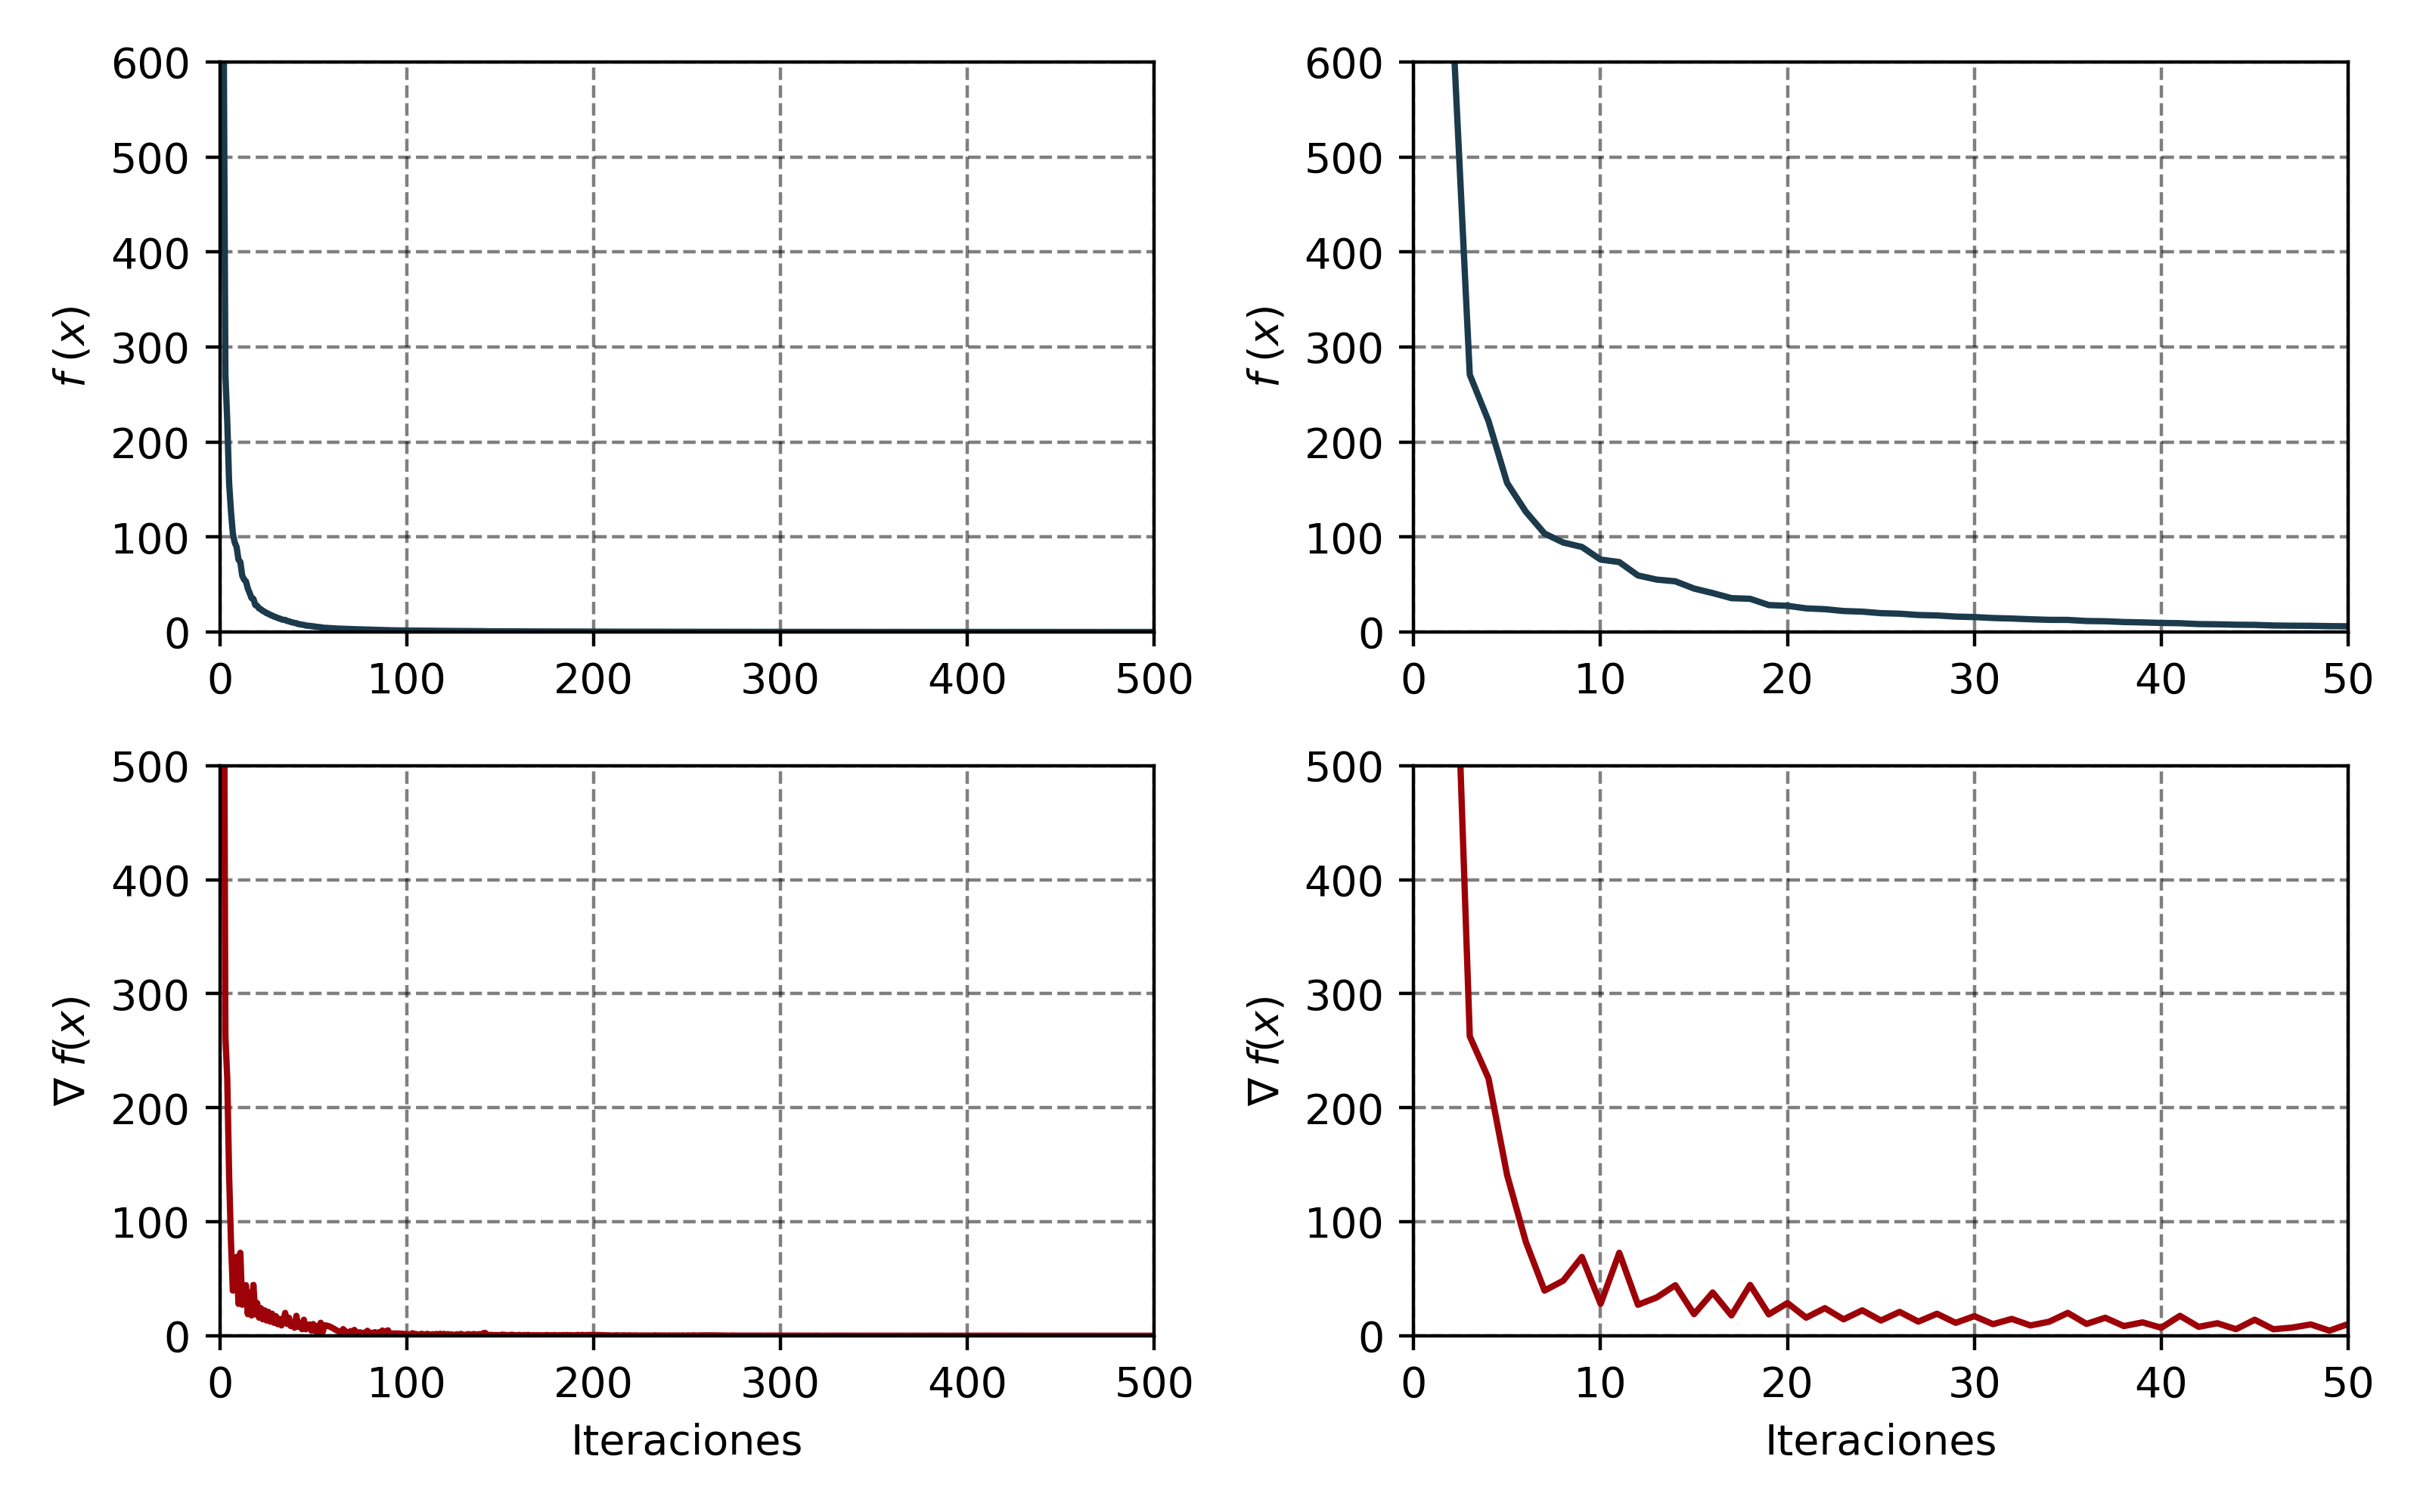
\includegraphics[width=14cm]{Graphics/log_likelihood_bisection.png}
    \caption{Resultados de la evaluación de la ecuación \ref{eq:log_likelihood_2} y la norma de la ecuación evaluada \ref{eq:grad_log_likelihood} en cada iteración realizada. De lado izquierdo se muestran los resultados hasta las 500 iteraciones y en en el lado derecho hasta las 50 iteraciones.}
    \label{fig:log_likelihood}
\end{figure}

Realizando el calculo del error que esta definido en la ecuación \ref{eq:error}. Se obtuvo que para el conjutno de datos de prueba es de 0.00047281.

\begin{equation}
    \text{error} = \frac{1}{n} \sum_{i=1}^n\left| 1_{\pi_i(\beta)>0.5(x_i)-y_i}\right|
    \label{eq:error}
\end{equation}